\section{Equivalent transformer}
\subsection{Circuit diagram}
\begin{figure}[H]
    \centering
    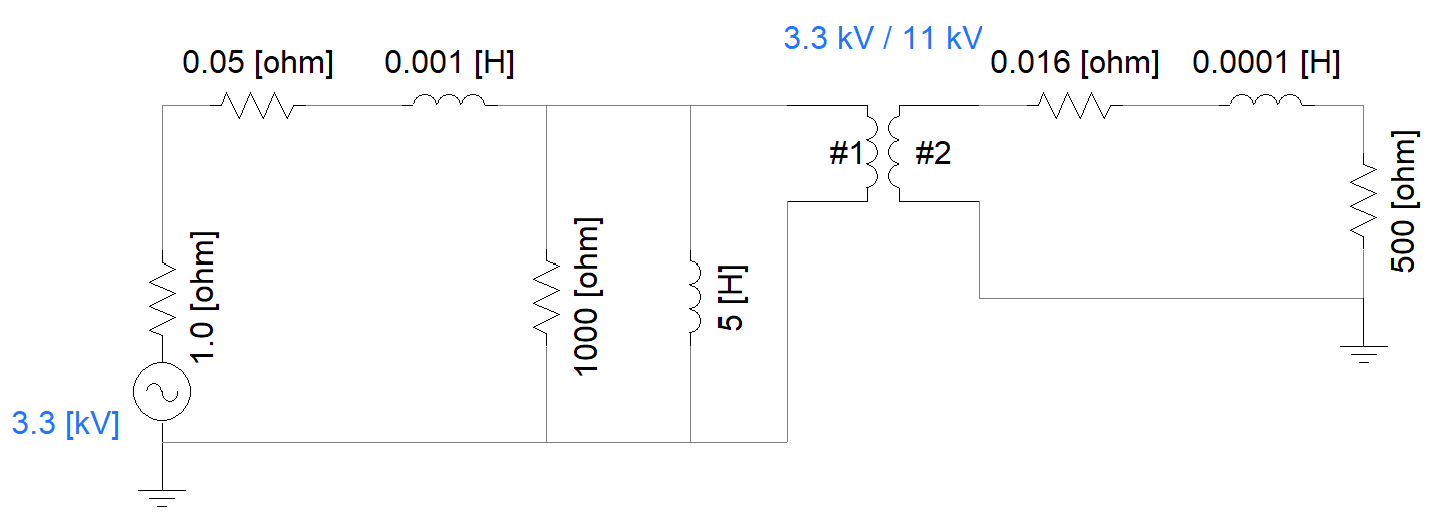
\includegraphics[width = \textwidth]{img/figure5.png}
    \caption{Circuit diagram to show equivalent transformer.}
    \label{fig:transformerCircuit}
\end{figure}
\subsection{RMS Voltage across the load}
Measuring the voltage across the load over \SI{0.1}{\second}, the voltage values were put into MATLAB (see Appendix \ref{app:q2}). The RMS voltage can be calculated using the following equation.
\begin{gather}
    V_{RMS} = \sqrt{\dfrac{\sum_{i=1}^n x_i^2}{n}}
\end{gather}
\begin{itemize}
    \item Number of data points ($n$): 401
    \item Number of complete AC cycles in time frame: 6
\end{itemize}
\begin{gather}
    V_{RMS,load} = \SI{10.72}{\kilo\volt}
\end{gather}